\section{Boundary Regret}
\label{sec:methodology}

The human signal $h$ shifts the model belief $b_x$ to the updated posterior $b_{x,h}$, but this shift carries decision value only when it moves $b_{x,h}$ across a decision facet---displacing the optimal action from $a_x$ to a rival.
Boundary regret measures exactly that displacement.

\begin{definition}[Boundary regret]\label{def:br-instance}
For an instance $x$ with model-optimal action $a_x$ and human signal $h$, the \emph{instance-level boundary regret} is
\[
    \BR(x, h) \;=\; V(b_{x,h}) \;-\; r_{a_x} \cdot b_{x,h}.
\]
This is the regret of keeping the model-only action $a_x$ after the belief updates from $b_x$ to $b_{x,h}$ (instantiating \texttt{regret} from \texttt{Regret.lean} at the model action and human-updated posterior).
\end{definition}

\begin{definition}[Ex ante boundary regret]\label{def:br-exante}
The \emph{ex ante boundary regret} at instance $x$ is
\[
    \BR(x) \;=\; \E_{h \mid x}[\BR(x, h)].
\]
This is the expected potential decision value of the human signal at instance $x$, before observing $h$.
\end{definition}

\begin{theorem}[VoI as Expected Boundary Regret]\label{thm:voi-br}
In any finite-action Bayesian decision problem with $a_x$ optimal at $b_x$,
\[
    \VoI(H \mid b_x)
    \;:=\; \E_h\bigl[V(b_{x,h})\bigr] - V(b_x)
    \;=\; \E_h\bigl[\BR(x, h)\bigr]
    \;=\; \BR(x).
\]
Formalized as \textup{\texttt{jensenGap\_eq\_weighted\_regret}} in \textup{\texttt{FacetActivation.lean}}.
\end{theorem}

\begin{proof}
The first equality is the definition of VoI.
For the second, apply the Bayesian martingale (Remark~\ref{rem:martingale}):
\[
    \E_h\bigl[r_{a_x} \cdot b_{x,h}\bigr]
    = r_{a_x} \cdot \E_h[b_{x,h}]
    = r_{a_x} \cdot b_x
    = V(b_x),
\]
where the last step uses the optimality of $a_x$ at $b_x$.
Subtracting from $\E_h[V(b_{x,h})]$:
\[
    \E_h\bigl[V(b_{x,h})\bigr] - V(b_x)
    = \E_h\bigl[V(b_{x,h})\bigr] - \E_h\bigl[r_{a_x} \cdot b_{x,h}\bigr]
    = \E_h\bigl[V(b_{x,h}) - r_{a_x} \cdot b_{x,h}\bigr].
    \qedhere
\]
\end{proof}

The proof is a direct algebraic consequence of the Bayesian martingale and the definition of regret.
We do not claim novelty for the VoI identity itself---it specializes results known in information economics \citep{RadnerStiglitz1984,DeLaraGossner2020}---but rather for the choice to package it as a deployment diagnostic for human--AI complementarity.

\begin{theorem}[Facet Activation Bridge]\label{thm:facet-bridge}
$\BR(x) > 0$ if and only if there exists a reachable posterior $b_{x,h}$ (i.e., $P(h \mid x) > 0$) and an action $a' \neq a_x$ such that
$r_{a'} \cdot b_{x,h} > r_{a_x} \cdot b_{x,h}$.
Equivalently, $\BR(x) = 0$ if and only if every reachable posterior remains in $\mathcal{R}_{a_x}$.

\smallskip\noindent
Formalized as \textup{\texttt{facet\_activation\_bridge}} in \textup{\texttt{FacetActivation.lean}};
the two directions also stand alone as
\textup{\texttt{jensenGap\_terminalValue\_zero\_of\_posteriors\_optimal}} and
\textup{\texttt{boundary\_crossing\_of\_strict\_jensenGap\_terminalValue}}.
\end{theorem}

\begin{proof}
By Theorem~\ref{thm:voi-br}, $\BR(x) = \E_h[\BR(x,h)]$.
Since $\BR(x,h) \geq 0$ for all $h$ (regret is non-negative), $\BR(x) > 0$ iff some $h$ with $P(h \mid x) > 0$ has $\BR(x,h) > 0$.
By definition, $\BR(x,h) > 0$ iff $V(b_{x,h}) > r_{a_x} \cdot b_{x,h}$, which holds iff some action $a'$ achieves $r_{a'} \cdot b_{x,h} > r_{a_x} \cdot b_{x,h}$.
The converse follows by contraposition: if $a_x$ is optimal at every reachable posterior, then $\BR(x,h) = 0$ for all $h$, hence $\BR(x) = 0$.
\end{proof}

\begin{corollary}\label{cor:zero-dv}
If every reachable human-updated posterior $b_{x,h}$ lies in $\mathcal{R}_{a_x}$, then $\VoI(H \mid b_x) = 0$, regardless of how much $H$ improves predictions as measured by log-loss, calibration, or any proper scoring rule.
\end{corollary}

\begin{figure}[t]
\centering
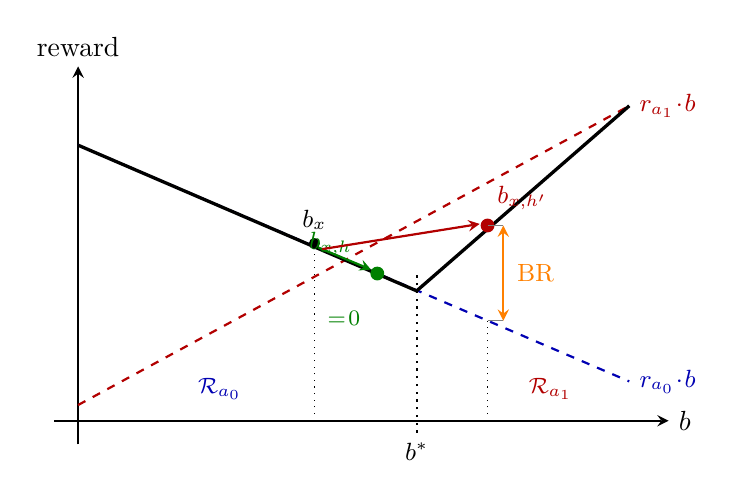
\begin{tikzpicture}[>=stealth, scale=1.0]
  % Axes
  \draw[thick,->] (-0.3,0) -- (7.5,0) node[right] {$b$};
  \draw[thick,->] (0,-0.3) -- (0,4.5) node[above] {reward};

  % Affine functions: r_{a_0} · b and r_{a_1} · b
  % a_0 (discharge): reward = 1-b mapped to (0,3.5) to (7,0.5)
  % a_1 (admit): reward = -4+5b mapped to (0,-1) to (7,3.5)
  % With x-axis = belief b ∈ [0,1] scaled to [0,7]

  % r_{a_0}: high at b=0, low at b=1
  \draw[dashed, blue!70!black, thick] (0,3.5) -- (7,0.5) node[right, font=\small] {$r_{a_0}\!\cdot\! b$};
  % r_{a_1}: low at b=0, high at b=1
  \draw[dashed, red!70!black, thick] (0,0.2) -- (7,4.0) node[right, font=\small] {$r_{a_1}\!\cdot\! b$};

  % V(b) = upper envelope
  \draw[very thick, black] (0,3.5) -- (4.3,1.65);
  \draw[very thick, black] (4.3,1.65) -- (7,4.0);

  % Decision facet (intersection)
  \draw[dotted, thick] (4.3,-0.15) -- (4.3,1.85);
  \node[below, font=\small] at (4.3,-0.15) {$b^*$};

  % Region labels
  \node[font=\footnotesize, blue!70!black] at (1.8, 0.4) {$\mathcal{R}_{a_0}$};
  \node[font=\footnotesize, red!70!black] at (6.0, 0.4) {$\mathcal{R}_{a_1}$};

  % Model belief b_x (in R_{a_0})
  \fill[black] (3.0, 2.25) circle (2pt);
  \node[above, font=\small] at (3.0, 2.3) {$b_x$};
  \draw[dotted, thin] (3.0,0) -- (3.0,2.25);

  % Posterior b_{x,h} still in R_{a_0}: no boundary crossing
  \fill[green!50!black] (3.8, 1.87) circle (2.5pt);
  \node[above left, font=\small, green!50!black] at (3.6, 1.97) {$b_{x,h}$};
  \draw[->, thick, green!50!black] (3.05, 2.2) -- (3.72, 1.92);
  % Mark BR = 0
  \node[font=\footnotesize, green!50!black] at (3.4, 1.3) {$\BR\!=\!0$};

  % Posterior b_{x,h'} crosses into R_{a_1}: boundary regret > 0
  \fill[red!70!black] (5.2, 2.48) circle (2.5pt);
  \node[above right, font=\small, red!70!black] at (5.2, 2.55) {$b_{x,h'}$};
  \draw[->, thick, red!70!black] (3.1, 2.18) -- (5.1, 2.5);

  % BR gap: V(b_{x,h'}) - r_{a_0} · b_{x,h'}
  % At x=5.2: r_{a_0} · b ≈ 3.5 - (3.0/7)*5.2 ≈ 3.5-2.23 = 1.27
  % At x=5.2: r_{a_1} · b ≈ 0.2 + (3.8/7)*5.2 ≈ 0.2+2.82 = 3.02
  % V = 3.02, r_{a_0} = 1.27, gap = 1.75 (too large, adjust)
  % Just mark the gap symbolically
  \draw[<->, thick, orange] (5.4, 1.27) -- (5.4, 2.48);
  \node[right, font=\small, orange] at (5.45, 1.88) {BR};

  % Dashed line from b_{x,h'} down to r_{a_0} level
  \draw[dotted, thin] (5.2, 0) -- (5.2, 1.27);
  \draw[thin, gray] (5.2, 1.27) -- (5.4, 1.27);
  \draw[thin, gray] (5.2, 2.48) -- (5.4, 2.48);
\end{tikzpicture}
\caption{
    Decision geometry for a two-action problem.
    $V(b)$ (solid) is the upper envelope of two affine reward functions (dashed).
    The decision regions $\mathcal{R}_{a_0}$ and $\mathcal{R}_{a_1}$ meet at the facet $b^*$.
    The model belief $b_x$ lies in $\mathcal{R}_{a_0}$.
    The posterior $b_{x,h}$ (green) remains in $\mathcal{R}_{a_0}$: the model action is still optimal and $\BR = 0$.
    The posterior $b_{x,h'}$ (red) crosses into $\mathcal{R}_{a_1}$: retaining $a_x = a_0$ incurs positive regret (orange gap).
    The green shift may improve predictions substantially yet have zero decision value; the red shift may improve predictions modestly yet carry positive decision value.
}
\label{fig:theory-geometry}
\end{figure}

Figure~\ref{fig:theory-geometry} illustrates the theorem geometrically.
A posterior that drifts within the incumbent region $\mathcal{R}_{a_x}$---no matter how large the log-loss improvement---contributes zero boundary regret and zero decision value.
Predictive expertise that does not cross a facet is invisible to the reward function.

\paragraph{Potential vs.\ realized value.}
$\BR(x)$ is an information-theoretic ceiling on the per-instance decision value of human review.
Realizing this value additionally requires correct elicitation, calibrated posterior updating, and operator compliance \citep{Vaccaro2024,BucinaEtAl2021}.
Boundary regret isolates the reward-local ceiling that any deferral policy or interface design must compete against.

\paragraph{Estimation.}
Theorems~\ref{thm:voi-br}--\ref{thm:facet-bridge} hold for any belief $b_x \in \Delta^{K-1}$; calibration is not a theoretical requirement.
In practice, the true belief $b_x$ is approximated by a (possibly imperfectly calibrated) model estimate (still written $b_x$ when the distinction is immaterial), and the true updated belief $b_{x,h}$ is approximated by $\bpost_{x,h} = P(Y \mid x, h)$ from a cross-fitted human-augmented model.
Calibration quality affects the accuracy of $\widehat\BR$ as an estimator of true boundary regret; Experiment~1 quantifies this sensitivity (Table~\ref{tab:exp1-calibration}).
We use the hat notation $\bpost$ throughout the experiments to distinguish estimated from exact posteriors.
The ex ante score $\widehat\BR_{\mathrm{pre}}(x)$ requires estimating $P(h \mid x)$ from training folds---before human review is observed---and computing $\widehat\E_{h \mid x}[V(\bpost_{x,h}) - r_{a_x} \cdot \bpost_{x,h}]$.
Section~\ref{sec:experiments} details the estimation pipeline for each experiment.
